\documentclass[12pt]{book}
\setlength{\parindent}{0pt}
%\setlength{\parskip}{1ex plus 0.5ex minus 0.2ex}
\usepackage[utf8]{inputenc}
\usepackage{graphicx}
\usepackage{rotating}

\usepackage[a4paper]{geometry}
\geometry{top=1.0in, bottom=1.0in, left=1.5in, right=1.0in}

\title{The DataTank\\
  \small A REST-ful webservice framework for PHP\\
  © iRail npo - CC By-Sa}
\author{
  Pieter Colpaert $<$pieter@iRail.be$>$\\
  Jan Vansteenlandt $<$jan@iRail.be$>$
}
\date{\today}
\begin{document}
\maketitle\setlength{\parindent}{0pt}
%\setlength{\parskip}{1ex plus 0.5ex minus 0.2ex}

%Set TOC page numbering to roman
\pagenumbering{roman}
\thispagestyle{empty}
\tableofcontents

%Write the preface here


%Normal pagenummering arabic
\pagenumbering{arabic}

%% TODO: split this into chapter files

%An introduction has to explain more about the title, and state 2 things: a mainproblem, and a subproblem.
%The document has to explain more about the architecture
\chapter{Introduction}

This document will explain the vision of the DataTank and outline the architecture.Note that as the DataTank is still under development, so is this document. We're trying hard to keep the documentation as up-to-date as possible. After all, a project's lifespan often depends on its documentation.

% SECTION 1: PHILOSOPHY
\chapter{Philosophy}
The DataTank is a platform that aims at making REST-ful API's as quick and easy as possible. Doing so, we want to enhance the ease of setting up API's build on open data and ease the search for certain datasets. The result of this platform will lead to a community of data providers (Back-end developers) and data consumers (App developers). The platform should also be able to identify certain datasets and establish relationships between them.

% SUBSECTION: DEV's VISION
\section{Developer vision}
\subsection{Problem}

Nowadays alot of data is available in a wide variety of dataformats. Finding certain data can be pretty hard, getting it in a certain dataformat could also be quite the job. If developers want to offer this data through a certain Web service API, they most likely have to set up everything from scratch. Errorhandling, requesthandling and documentation are just some of the jobs that have no direct link with setting up a working API for data consumers. Wouldn't it be great that a developer could just implement its call and its return object and could somewhat automize everything else? ...That's exactly what the DataTank wants to achieve for developers.

Our platform offers API builders an environment in which they can put their focus mostly on handling a call and returning an answer. One of the biggest headaches in implementing the business logic is handling errors. Our platform offers several prebuild exception objects that can be used in handling errors of a call, the only thing that needs to be done is identify what exception seems fit and throwing it. The handling of this exception and the logging, will be performed by the platform. If the developer doesn't find a fitting exception he can ofcourse implement it's own exception.

One of the most important things a good API needs is documentation. Besides handling a call, the developer must also document its Web service. The platform will automatically pick up the documentation for a certain call and puts it in the documentation webpage of the DataTank.
Next to a semi automated set up of an API, the platform also offers some basic analysis tools for back-end developers. These tools display the errors and number of requests in a certain period to a certain API method at your command.

% SUBSECTION APP'S VISION
\section{App builder vision }
Currently we're in the middle of revolution in which people have access to as much information they want, whenever they want and wherever they want it. App developers are always on the lookout for new information or brainstorming about the next big idea for an app. The DataTank will offer these builders a quick overview of all the registered datasets available, and the necessary documentation. Not only is this very useful for developing purposes but also for brainstorm sessions about how certain data can be used in an original way.

\section{Global vision} 
It's always nice to create some sort of global future vision and implement ideas on how to achieve that vision. With the DataTank we want it to be as easy as possible to offer open data in an API. Next to that we want different datasets to be combinable. (i.e. If you want to calculate a route from A to B it might be helpful to get a dataset involving trains as well as a dataset involving busses). 

Everyone can set up its own "local" DataTank. All these local DataTanks will communicate with the "global" DataTank. The back-end developer and/or app developer can set up its own DataTank, containing a few datasets it wants to offer and use. This will be picked up by our global DataTank so that others can find datasets they are looking for and use them. This will lead to a more distributed dataplatform in which everyone (developers and app builders) will find what they need. In a very simplistic way the DataTank could be considered a portal for datasets. Actually it's more then your average portal website. The DataTank itself will handle calls and return a result. If the DataTank was a normal portal site it would just redirect you to a different website, namely the one where the API was hosted.

% SECTION: ARCHITECTURE
\chapter{Architecture}
\begin{sidewaysfigure}[H]
  \centering
  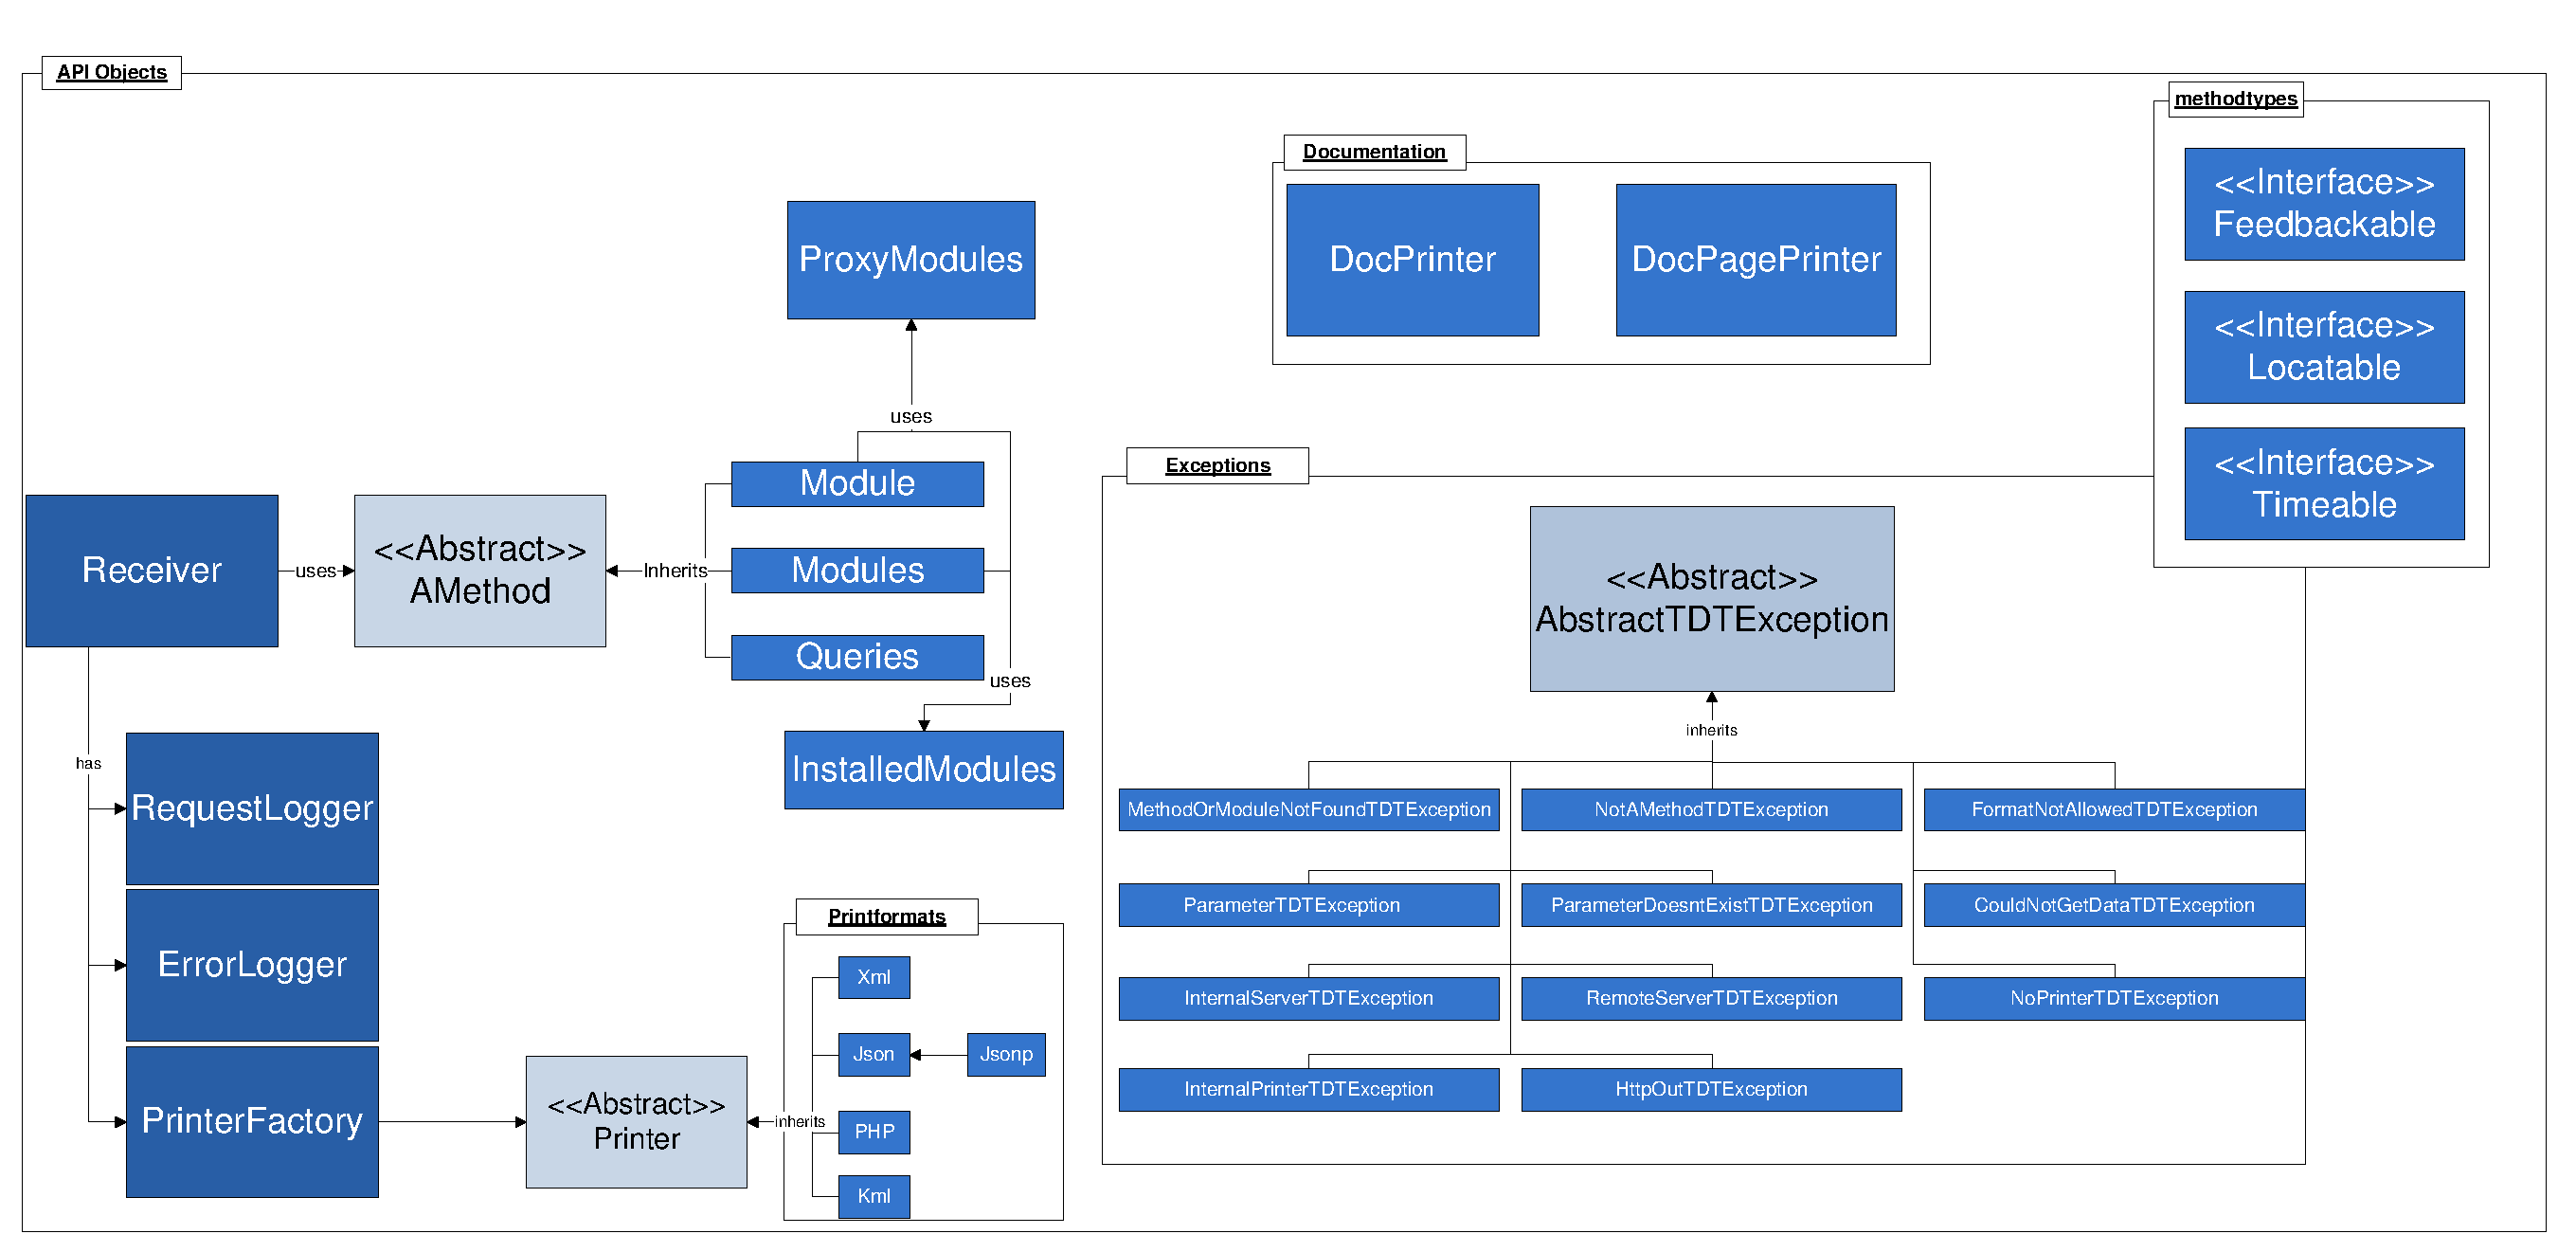
\includegraphics[scale=0.4]{graphics/UMLModelTDT.pdf}
  \caption{Architecture}
  \label{fig:Architecture}
\end{sidewaysfigure}
\begin{sidewaysfigure}[H]
 \centering
 \includegraphics[scale=0.5]{graphics/FlowchartTDT.pdf}
 \caption{Workflow of the DataTank}
 \label{fig:workflow}
\end{sidewaysfigure}
\chapter{Near future work}
\end{document}
